\documentclass[10pt]{beamer}
\usepackage{tikz} % For handling images in the background
\usepackage{graphicx} % For including images
\usepackage{amsmath}
\usepackage{bigints}



\usetheme[progressbar=frametitle]{metropolis}
\usepackage{appendixnumberbeamer}

\usepackage{booktabs}
\usepackage[scale=2]{ccicons}

\usepackage{pgfplots}
\usepgfplotslibrary{dateplot}
%\institute{A.A. }
\usepackage{xspace}
\newcommand{\themename}{\textbf{\textsc{metropolis}}\xspace}


% Customize the frametitle area with an image and move it to the bottom
% Redefine the frame title template for a custom bottom frame with an image
\definecolor{rugred}{rgb}{0.17,0,0.34}
\colorlet{rugred_less}{rugred!15!white}
%\setbeamertemplate{frametitle}{fg=white,bg=rugred}

\setbeamertemplate{footline}{
    \begin{beamercolorbox}[wd=\paperwidth,ht=4ex,dp=2.5ex,center]{author in head/foot} % Footline height adjusted
        \usebeamerfont{author in head/foot} 
        \small % Change font size for author, institution, and page number
        \insertshortauthor % Author text
        \hspace{0cm} % Space between author and institution
        \textbar \hspace{1.5cm} % Optional separator between author and institution (using a bar)
        A.A. 2024-25 % Institution text
        \hspace{1.5cm}\textbar\hspace{2.8cm} % Space between institution and page number
        \insertframenumber % Page number aligned to the right
    \end{beamercolorbox}
}



\setbeamercolor{title}{fg=rugred} % Main title text becomes green
\setbeamercolor{author}{fg=rugred} % Main title text becomes green
\setbeamercolor{date}{fg=rugred} % Main title text becomes green
\setbeamercolor{background canvas}{bg=white}

\setbeamercolor{titlelike}{fg=rugred}
\setbeamercolor{section in toc}{fg=rugred}
\setbeamercolor{item}{fg=rugred}
\setbeamercolor{block title}{fg=white,bg=rugred}

\setbeamercolor{block body}{fg=black,bg=rugred_less}
\setbeamercolor{alerted text}{fg=rugred}

\setbeamercolor{palette primary}{bg=rugred,fg=white}
\setbeamercolor{frametitle}{bg=rugred}

\title{Bayesian physical reconstruction of initial conditions from large-scale structure surveys}
\subtitle{\small\textit{paper by Jens Jasche \& Benjamin D. Wandelt}}
% \date{\today}
\date{12/02/25}
\author{Lorenzo Cavezza - 2130648}

\titlegraphic{\hfill
\includegraphics[height=1.5cm]{2022_pod.png}}
%\setlength{\columnsep}{0.1cm} % Adjust column spacing

\begin{document}

\maketitle

\begin{frame}{Table of contents}
  \setbeamertemplate{section in toc}[sections numbered]
  \tableofcontents%[hideallsubsections]
\end{frame}

\section[Introduction]{Introduction}

\begin{frame}[fragile]{LSS analysis}

\begin{columns}
        \begin{column}{0.6\textwidth} % Left column (text)
         %\metroset{block=fill}
\begin{block}<1->{Standard Approach}

\begin{itemize}
        \item<1-> \alert<1> {Tracers' Surveys (Galaxy Surveys)}
        \item<2-> \alert<2> {Initial Conditions Constraining}
        \item<3-> \alert<3> {Evolved Density Field Approximations}
\end{itemize} 
\end{block}

        \end{column}\\
        \begin{column}{0.4\textwidth} % Right column (image)
        \begin{center}
            \includegraphics<1->[width=0.8\textwidth]{Sloan_Digit_Sky_Survey_1.25_Declination_Slice_2013_720.jpg}\end{center}

        \end{column}
    \end{columns}\pause
   \begin{block}<4->{Proposed Alternative}
\begin{itemize}
        \item<4-> \alert<4> {2LPT dynamically evolved final density field prior}
        \item<5-> \alert<5> {Hamiltonian Monte Carlo exploration of initial field conditioned on mock observations}
\end{itemize} 
\end{block} 
\end{frame}
\section[Bayesian Framework]{Bayesian Framework}


\begin{frame}[fragile]{The non - Gaussian Prior}
Given a model of \textbf{LSS} formation $G\left(a,\delta^i\right)$ (a \textit{Second Order Lagrangian Perturbation Thoery} model (\textbf{2LPT}) in our case), we obtain the final density contrast $\delta^f$ prior as:\\
\begin{center}
    \begingroup\makeatletter\def\f@size{9}\check@mathfonts
$\mathcal{P}\left(\{\delta_l^f\}\right)=\bigintsss d\{\delta_l^i\}\mathcal{P}\left(\left\{\delta_l^i\right\},\left\{\delta_l^f\right\}\Bigm| \textbf{S}\right)=$
\endgroup
\hfill

\pause
\begingroup\makeatletter\def\f@size{9}\check@mathfonts
$ =\bigintsss d\{\delta_l^i\}\mathcal{P}\left(\left\{\delta_l^f\right\}\Bigm|\left\{\delta_l^i\right\} \right)\mathcal{P}\left(\left\{\delta_l^i\right\}\Bigm| \textbf{S}\right)=$
\endgroup
\hfill

\pause

\begingroup\makeatletter\def\f@size{9}\check@mathfonts
$ =\bigintsss d\{\delta_l^i\}\prod\limits_l\delta^D\left(\delta_l^f-G\left(a,\delta^i\right)_l\right)\left(\frac{e^{-\frac{1}{2}\sum_{lm}\delta_l^i\textbf{S}_{lm}^{-1}\delta_m^i}}{det\left(2\pi\textbf{S}\right)}\right)$\endgroup
\end{center}
\pause
with \textbf{S} representing the initial contrast covariance matrix. \\
\hfill\\
This can be done through sampling of $\mathcal{P}\left(\left\{\delta_l^f\right\},\left\{\delta_l^i\right\}\Bigm| \textbf{S}\right)$ and discarding the $\delta_l^i$ realization
\end{frame}
\begin{frame}[fragile]{The LSS Likelihood}
We can model the observed tracers, namely galaxies, through an 
\textit{inhomogeneous \textbf{Poisson} Likelihood}:\begin{center}
$\mathcal{P}\left(\{N_k^g\}\Bigm |\{\lambda_k\}\right)=\prod\limits_k\frac{\left(\lambda_k\right)^{N_k^g}e^{-\lambda_k}}{N^g_k!}$\end{center}\pause
  with \begin{itemize}
      \item $N_k^g$: observed galaxy number at position $x_k$
      \item $\lambda_k$: expected galaxy number at $x_k$:
      \begin{center}
  $\lambda_k=\lambda_k(\delta)=R_k\overline{N}\left(1+B(\delta^f)_k\right)$
  \end{center}\pause
  where:
  \begin{itemize}
      \item $R_k$: survey geometries and selection functions linear operator
      \item $B(x)_k$: non linear and non local bias operator
  \end{itemize}
  \end{itemize}
  

\end{frame}
\begin{frame}[fragile]{The 2LPT - Poisson Posterior}
The joint posterior of the final and initial contrast densities is:
\begin{center}
\begingroup\makeatletter\def\f@size{9}\check@mathfonts
$\mathcal{P}\left(\left\{\delta_l^f\right\},\left\{\delta_l^i\right\}\Bigm|\left\{N_i\right\}, \textbf{S}\right)=$
\endgroup
\hfill

\pause

\begingroup\makeatletter\def\f@size{6}\check@mathfonts
$=\prod\limits_k\frac{\left(\lambda_k\left(\delta^f\right)\right)^{N_k^g}e^{-\lambda_k\left(\delta^f\right)}}{N_k^g!}$\endgroup
\begingroup\makeatletter\def\f@size{7}\check@mathfonts
$\prod\limits_l\delta^D\left(\delta_l^f-G\left(a,\delta^i\right)_l\right)\left(\frac{e^{-\frac{1}{2}\sum_{lm}\delta_l^i\textbf{S}_{lm}^{-1}\delta_m^i}}{det\left(2\pi\textbf{S}\right)}\right)$\endgroup

\end{center}\pause
which leads to the marginalized initial density posterior:\begin{center}
$\mathcal{P}\left(\left\{\delta_l^i\right\}\Bigm|\left\{N_i\right\}, \textbf{S}\right)=\prod\limits_k \frac{\left(\lambda_k\left(G\left(a,\delta^i\right)\right)\right)^{N_k^g}e^{-\lambda_k\left(G\left(a,\delta^i\right)\right)}}{N_k^g!}\left(\frac{e^{-\frac{1}{2}\sum_{lm}\delta_l^i\textbf{S}_{lm}^{-1}\delta_m^i}}{det\left(2\pi\textbf{S}\right)}\right)$
\end{center}\pause
Benefits: 
\begin{itemize}
    \item Forward Model Evaluation
    \item All uncertaintes accounted (survey geometry, selection biases, galaxy distribution noise and cosmic variance)
\end{itemize}
\end{frame}
\section[Hamiltonian Monte Carlo]{HMC}

\begin{frame}[fragile]{Hamiltonian Monte Carlo}

\begin{itemize}
   \item Why \textit{HMC}?\pause
   \begin{itemize}
    \item[$\implies$] $2\cdot10^6$ parameters to infer (box's voxels) $\implies$ very low acceptance in random walk based MC (\textit{curse of dimensionality})\pause
    \item[$\implies$] \textit{HMC} yields an acceptance of nearly 1 (integration errors)
    \end{itemize}\pause
    \item \textit{HMC} moves smoothly inside \textit{typical volumes} by exploiting well defined equations of motion through the \textit{Hamiltonian}:
    \begin{center}
        $H=\sum\limits_i\sum\limits_j\frac{1}{2}p_i\textbf{M}_{ij}^{-1}p_j + \psi\left(x\right) = \sum\limits_i\sum\limits_j\frac{1}{2}p_i\textbf{M}_{ij}^{-1}p_j -\ln{\mathcal{P}\left(x\right)} $
         \pause
    $\implies e^{-H}=\mathcal{P}\left(\{x_i\}\right)exp\left(-\frac{1}{2}\sum\limits_i\sum\limits_j p_i\textbf{M}_{ij}^{-1}p_j \right)$\end{center}\pause
    \item Momenta randomly drawn and easily marginalized as nuisance parameters. After dynamical evolution the \textit{acceptance probability} is
    \begin{center}
            \begingroup\makeatletter\def\f@size{10}\check@mathfonts

    $\mathcal{P}_A = \min \left[1,\exp{\left(-\left(H\left(\{x_i'\},\{p_i'\}\right)-H\left(\{x_i\},\{p_i\}\right)\right)\right)}\right]$
    \endgroup
\end{center}
\end{itemize}



 
\end{frame}

\begin{frame}[fragile]{LSS Equations of Motion}

We get the Equations of Motion through \textit{Hamilton's equations}:\pause
\begin{center}

\begingroup\makeatletter\def\f@size{8}\check@mathfonts
    $\frac{d\delta_n^i}{dt}=\frac{\partial H}{\partial p_i}=\sum\limits_j\textbf{M}_{nj}^{-1}p_j$
    \endgroup
    \hspace{0.3cm} with\hspace{0.3cm}
    \begingroup\makeatletter\def\f@size{8}\check@mathfonts
$\textbf{M}_{nj}=\textbf{S}_{nj}^{-1}-\delta_{nj}^KD^1\left\frac{\partial \textbf{J}_j(s)}{\partial s_j}\right\rvert_{s_j=\xi_j}$
    \endgroup\\

\end{center}\pause
The Hamiltonian mass optimizes the integrator's stability . Vector $\textbf{J}$ accounts for the gradient of the first order approximate \textit{"Zeldovich"} potential.\pause
We define the potential of the Hamiltonian system explicitely:
\begin{center}
    \begingroup\makeatletter\def\f@size{8}\check@mathfonts
    $\textbf{$\Psi$}\left(\{\delta_l^i\}\right)=-\ln{\left(\mathcal{P}\left(\{\delta_l^i\Bigm|\{N_i\},\textbf{S}\}\right)\right)}$    \endgroup\pause
 \begingroup\makeatletter\def\f@size{10}\check@mathfonts
 $=\textbf{$\Psi$}_{prior}\left(\{\delta_l^i\}\right)+\textbf{$\Psi$}_{likelihood}\left(\{\delta_l^i\}\right)=$
    \endgroup
    \end{center}
\pause
    \begin{center}

\begingroup\makeatletter\def\f@size{8}\check@mathfonts
    $=\frac{1}{2}\sum\limits_{lm}\delta_l^i\textbf{S}_{lm}^{-1}\delta_m^i+\sum\limits_k\left[R_k\bar{N}\left(1+G\left(a,\delta^i\right)_k\right)-N_k\ln{\left(R_k\bar{N}\left(1+G\left(a,\delta^i\right)_k\right)\right)}\right]$    
    \endgroup

\pause

\begingroup\makeatletter\def\f@size{10}\check@mathfonts
   $\implies\textbf{$\frac{dp_n^i}{dt}$}=-\frac{\partial\textbf{$\Psi$}_{prior}\left(\{\delta_l^i\}\right)}{\partial\delta_p^i}-\frac{\partial\textbf{$\Psi$}_{likelihood}\left(\{\delta_l^i\}\right)}{\partial\delta_p^i}=$
   \endgroup
   \hfill\\
   \pause
   
   \begingroup\makeatletter\def\f@size{8}\check@mathfonts
   $=-\sum\limits_j\textbf{S}_{pj}^{-1}\delta_j^i+D^1J_n-D^2\sum\limits_{a>b}\left(\tau_n^{aabb}-\tau_n^{bbaa}-2\tau_n^{abab}\right)$
    \endgroup
\end{center}
where the $\tau_m^{abcd}$ accounts for the gradient of the second order lagrangian potential.
\end{frame}

\begin{frame}[fragile]{The Leapfrog Method}
As an integration scheme the Leapfrog Method is used:\\
$\implies$ simplest integration method that conserves the energy and phase space area and is time reversible \pause
\begin{columns}
        \begin{column}{0.5\textwidth} % Left column (text)
        \begingroup\makeatletter\def\f@size{7}\check@mathfonts

        $p_m\left(t+\frac{\epsilon}{2}\right)=\left.p_m(t)-\frac{\epsilon}{2}\frac{\partial\psi\left(\{\delta_k^i\}\right)}{\delta_l^i}\right\rvert_{\delta_m^i(t)}$
$\delta_m^i\left( t+\epsilon\right)=\delta_m^i(t)-\frac{\epsilon}{m_i}p_m\left(t+\frac{\epsilon}{2}\right)$
$p_m\left(t+\epsilon\right)=\left.p_m\left(t+\frac{\epsilon}{2}\right)-\frac{\epsilon}{2}\frac{\partial\psi\left(\{\delta_k^i\}\right)}{\delta_l^i}\right\rvert_{\delta_m^i(t+\epsilon)}$   \endgroup
\end{column}
        \begin{column}{0.5\textwidth} % Right column (image)
            \includegraphics[width=\textwidth]{Schematics-describing-how-the-leapfrog-algorithm-works-Position-and-velocity-leap-each.png}
        \end{column}
    \end{columns}
    \pause
which translates to:
\begin{center}
\begingroup\makeatletter\def\f@size{10}\check@mathfonts
   $p_m(t+\epsilon) = p_m(t) - \frac{\epsilon}{2}\left(\left\frac{\partial\Psi(\delta^i)}{\partial\delta_i^i}\right\rvert_{\delta^i(t)}+\left\frac{\partial\Psi(\delta^i)}{\partial\delta_m^i}\right\rvert_{\delta^i(t+\epsilon)}\right)$
   \endgroup
   
   \begingroup\makeatletter\def\f@size{10}\check@mathfonts
   $\delta_m(t+\epsilon) = \delta_m(t) + \epsilon\sum\limits_j\textbf{$M$}_{mj}^{-1}p_j(t)-\frac{\epsilon^2}{2}\sum\limits_j\textbf{$M$}_{mj}^{-1}\left\frac{\partial\Psi(\delta^i)}{\partial\delta^i_j}\right\rvert_{\delta^i(t)}$
   \endgroup
\end{center}




  
\end{frame}
\section[Testing the Model]{Testing}
\begin{frame}[fragile]{Mock Observations}

  \begin{columns}
        
        \begin{column}{0.3\textwidth} % Right column (image)
            
            \begin{tikzpicture}[node distance=1.1cm]

% Define the styles for the nodes and the arrow
\tikzstyle{box} = [rectangle, draw, minimum width=3cm, minimum height=0.8cm, text centered, fill=rugred_less]
\tikzstyle{arrow} = [thick,->,>=stealth]

% Draw the boxes and connect them
\node (box1)[box]  {$\delta_i$ Generation}\pause;
\draw[arrow]  (box1) -- (box2);
\node (box2) [box, below of=box1] {Expansion by $D^+$}\pause;
\draw [arrow] (box2) -- (box3);
\node (box3) [box, below of=box2] {2LPT Propagation}\pause;
\draw [arrow] (box3) -- (box4);
\node (box4) [box, below of=box3] {Galaxy Sowing}\pause;
\draw [arrow] (box4) -- (box5);
\node (box5) [box, below of=box4] {Sloan Mask}\pause;
\draw [arrow] (box5) -- (box6);
\node (box6) [box, below of=box5] {Schechter Selection}\pause;






\end{tikzpicture}
        \end{column}
        \begin{column}{0.7\textwidth} % Left column (text)
        \begin{columns}
                    \begin{column}{0.5\textwidth} % Left column (text)
                    \includegraphics<5->[width=1\textwidth]{stt449fig2.jpeg}
\end{column}
\begin{column}{0.6\textwidth} % Left column (text)
\includegraphics<6->[width=1\textwidth]{stt449fig1.jpeg}

\end{column}
        \end{columns}
            \begin{center}
            
            \begingroup\makeatletter\def\f@size{9}\check@mathfonts \uncover<6->{with:
                $f(z)=\frac{\int_{M_{min}(z)}^{M_{max}(z)}\Phi(M)dM}{\int_{M_{min}}^{M_{max}}\Phi(M)dM}$
                \endgroup}
            \end{center}
            
            \uncover<6->{where $\Phi(M)$ is the \textit{Schechter} luminosity function.}\uncover<7->{
            The linear operator used in Poisson Sampling is:}
             \begin{center}
                    \begingroup\makeatletter\def\f@size{8}\check@mathfonts
                \uncover<7->{{$R_i=M_iF_i=M(\alpha_i,\delta_i)f^l(z_i)$}}
                \endgroup
            \end{center}
        \end{column}
    \end{columns}

\end{frame}
\begin{frame}[fragile]{Burn - In}

 \begin{columns}
        \begin{column}{0.7\textwidth} % Left column (text)
         \begin{itemize}
             \item Arbitrarily lower strength $\delta_l^i$ by one tenfold
             \item Quantify power spectra drift with:
             \begin{center}
        \begingroup\makeatletter\def\f@size{10}\check@mathfonts
            $\xi\left(P_i(K)\right)=1-\frac{P_i(k)}{P^0(k)}$
            \endgroup
        \end{center}\pause
         \end{itemize} 
        \end{column}\\
        \begin{column}{0.35\textwidth} % Right column (image)
            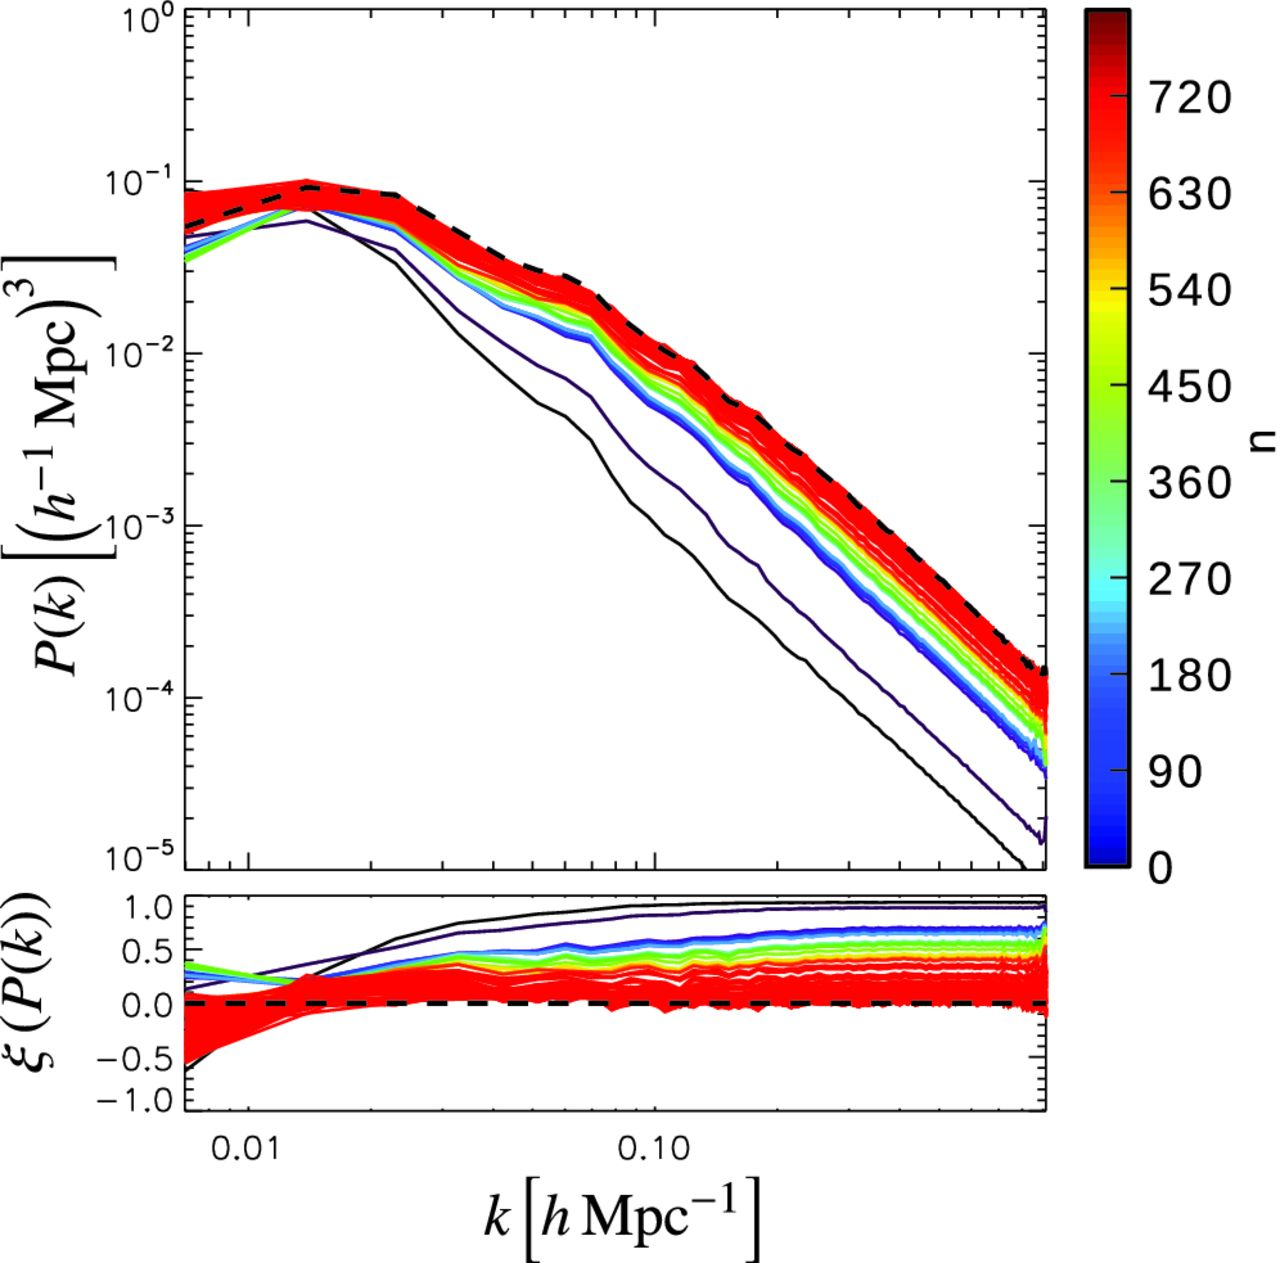
\includegraphics[width=1.1\textwidth]{stt449fig11.jpeg}

        \end{column}
    \end{columns}\pause
 \begin{columns}
 \begin{column}{0.35\textwidth} % Right column (image)
            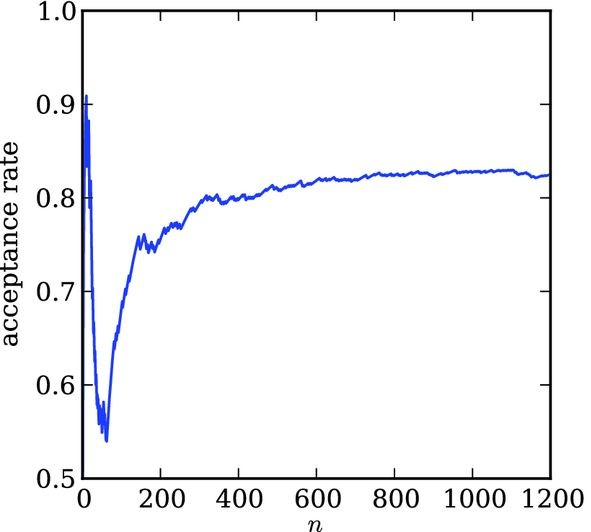
\includegraphics[width=1\textwidth]{stt449fig3_half.jpeg}

        \end{column}
        \begin{column}{0.7\textwidth} % Left column (text)
        
        \begin{itemize}
            \item Acceptance takes a dip after manual drift
            \item Back to normal ($\sim$ 84\%) after $\sim$ 600 epochs
        \end{itemize}
        \end{column}
        
    \end{columns}


  
\end{frame}
\begin{frame}[fragile]{Autocorrelation}


   \begin{columns}
   
        \begin{column}{0.7\textwidth} % Left column (text)
        Autocorrelation is computed to determine the number of independent samples and to assess good mixing:
        \begin{center}
        \begingroup\makeatletter\def\f@size{8}\check@mathfonts

$C(\delta)_n=\left\langle\frac{\delta^i-\langle\delta\rangle}{\sqrt{Var\left(\delta\right)}}\frac{\delta^{i+n}-\langle\delta\rangle}{\sqrt{Var\left(\delta\right)}}\right\rangle$
\end{center}
\endgroup\pause
We see such correlations plotted from different signal-to-noise ratios $\sqrt{N}$
        \end{column}
        \begin{column}{0.4\textwidth} % Right column (image)
            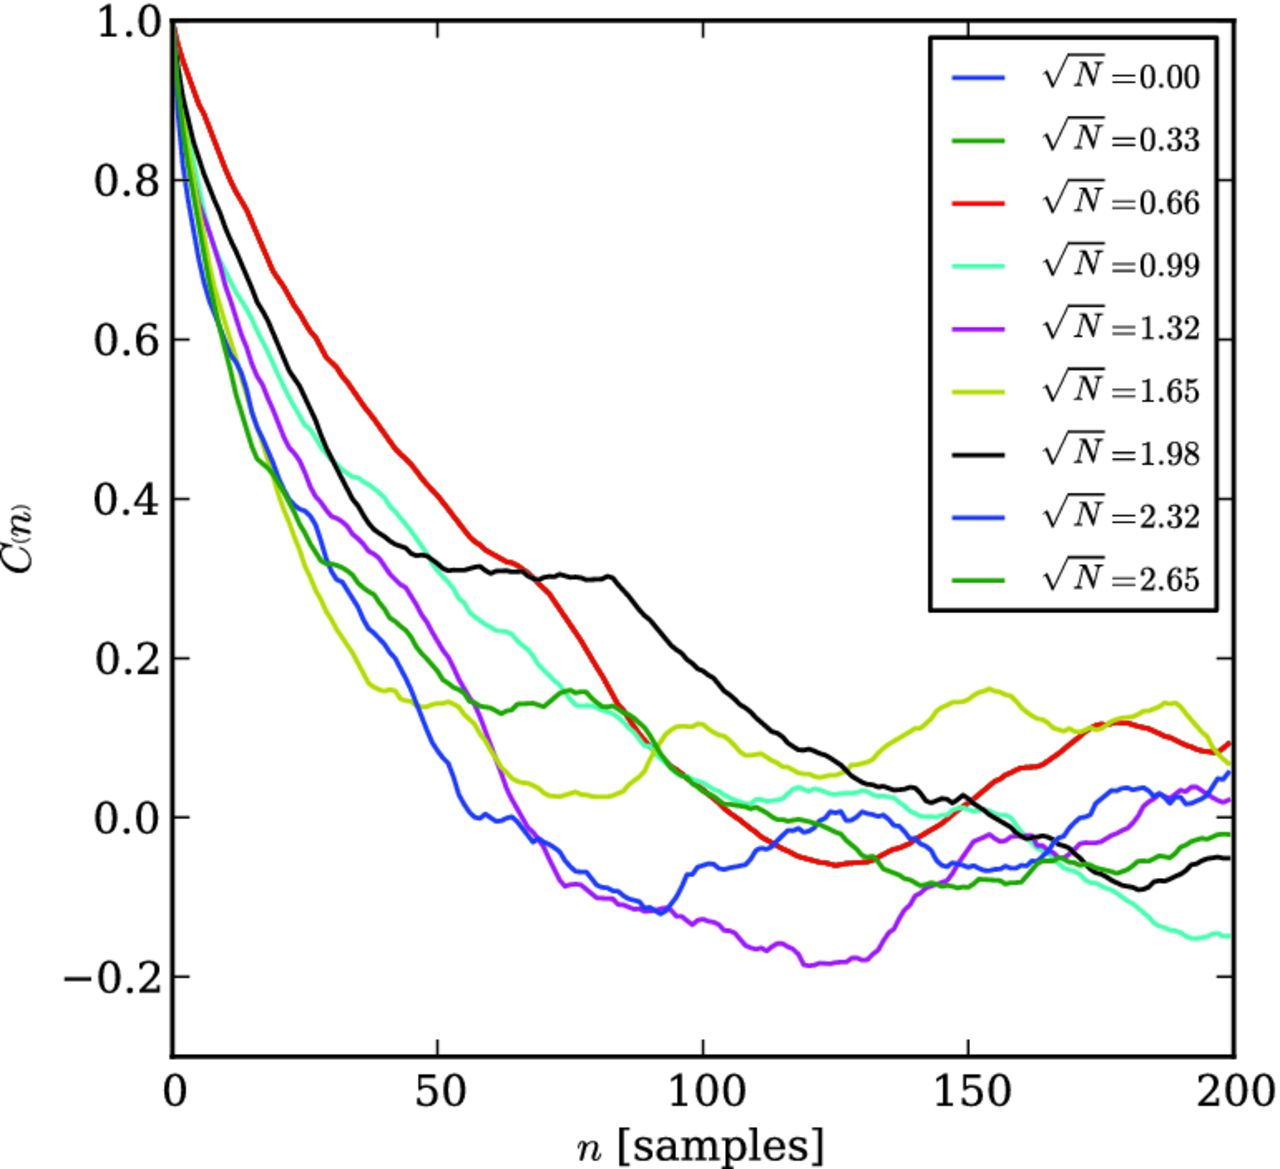
\includegraphics[width=\textwidth]{stt449fig4.jpeg}
        \end{column}
    \end{columns}
    \begin{center}
    $C(\delta)_n < 0.1$ when $n\sim200 \implies$ correlation length is about $200$
    \end{center}
\end{frame}
\begin{frame}[fragile]{Inferred Density Fields}
Samples from the sampled density fields and mock data:
\begin{columns}
        \begin{column}{0.7\textwidth} % Right column (image)
            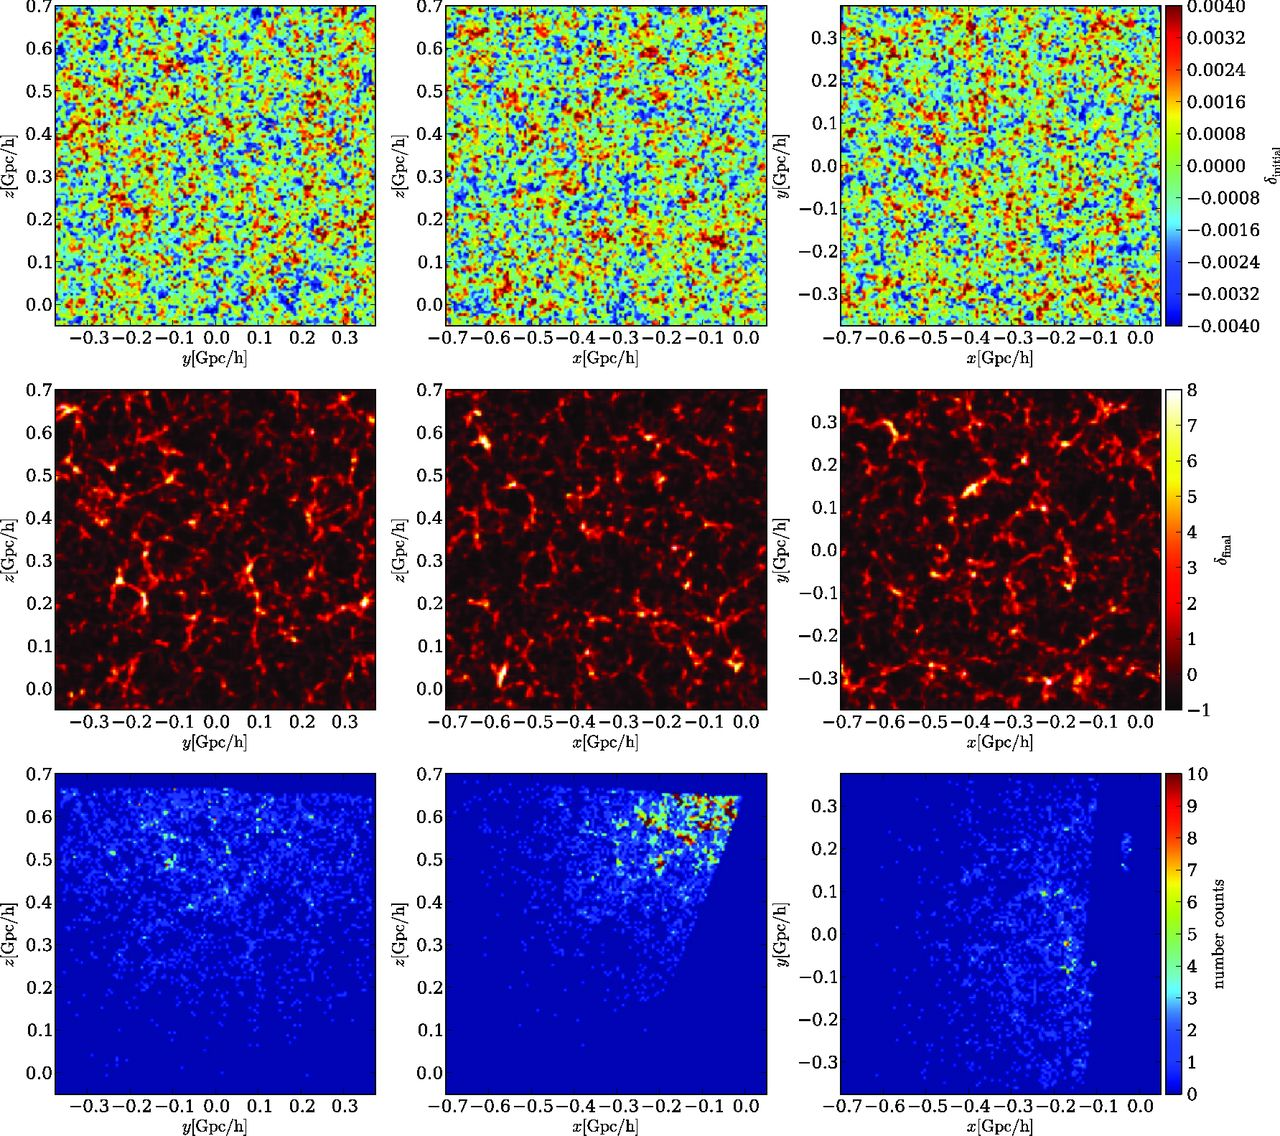
\includegraphics[width=1.1\textwidth]{stt449fig5.jpeg}
        \end{column}\pause
        \begin{column}{0.2\textwidth} % Right column (image)
            \includegraphics[width=1.15\textwidth]{0911.2498v1_page-0004.jpg}
        \end{column}
\end{columns}
  
\end{frame}

\begin{frame}[fragile]{Inferred Density Fields}
One-point distribution of density contrasts:

 
\begin{center}
            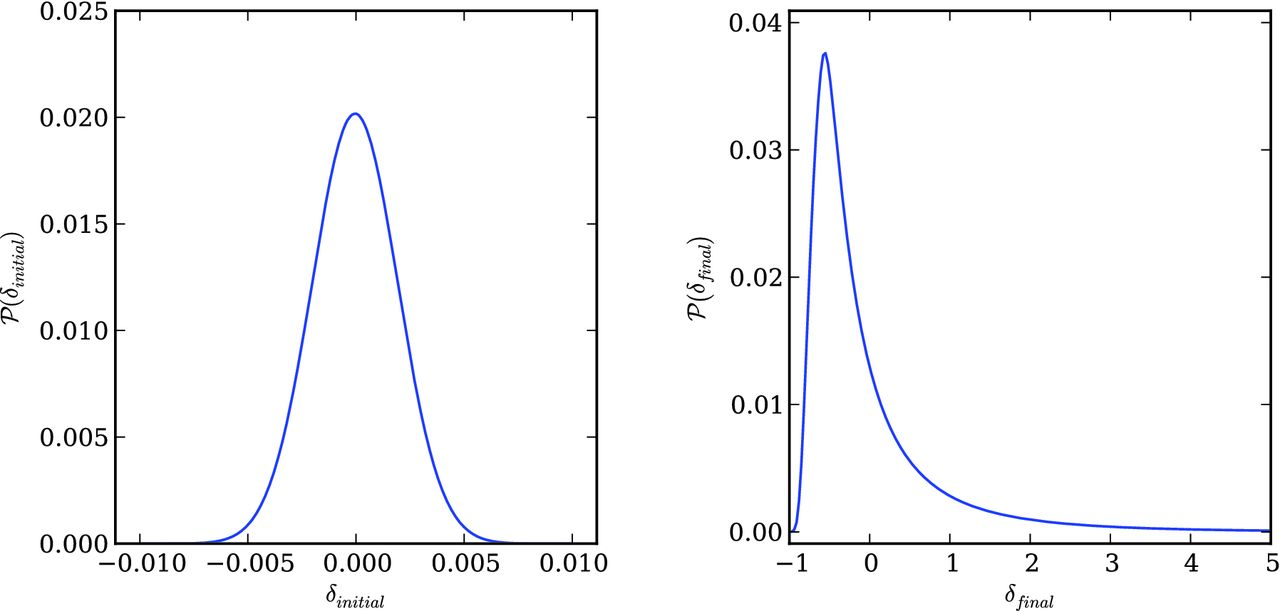
\includegraphics[width=1\textwidth]{stt449fig7.jpeg}

\end{center}
  
\end{frame}
\begin{frame}[fragile]{Accuracy}
   \begin{columns}
 \begin{column}{0.65\textwidth} % Left column (text)
 Inferred initial density accuracy is assessed with the posterior of $\tiny\Delta\delta_{initial}=\delta_{initial}^{true}-\delta_{initial}$\ conditioned to a signal-to-noise ratio proxy:
 \begin{center}
\begingroup\makeatletter\def\f@size{11}\check@mathfonts
$\Sigma=\frac{\lvert\langle\delta_{initial}\rangle\rvert}{\sqrt{\langle\left(\delta_{initial}-\langle\delta_{initial}\rangle\right)^2\rangle}}$
\endgroup
\end{center}
        \end{column}
        \begin{column}{0.3\textwidth} % Right column (image)
            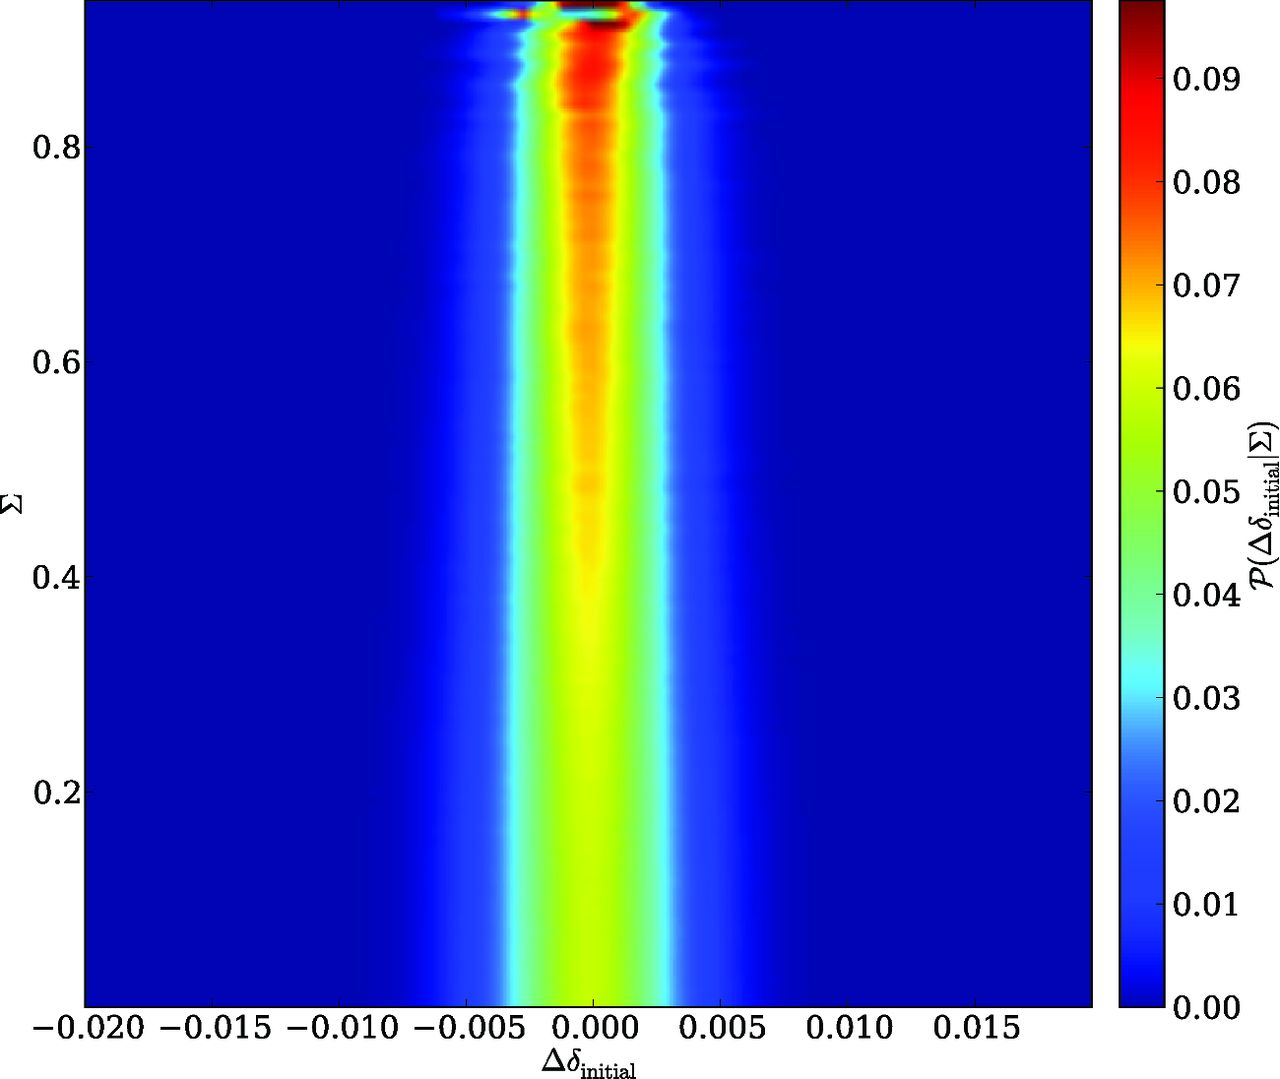
\includegraphics[width=1.15\textwidth]{stt449fig8.jpeg}
        \end{column}
    \end{columns}
    \hfill
    \hspace{1cm}\pause
   \begin{columns}
 \begin{column}{0.5\textwidth} % Left column (text)
  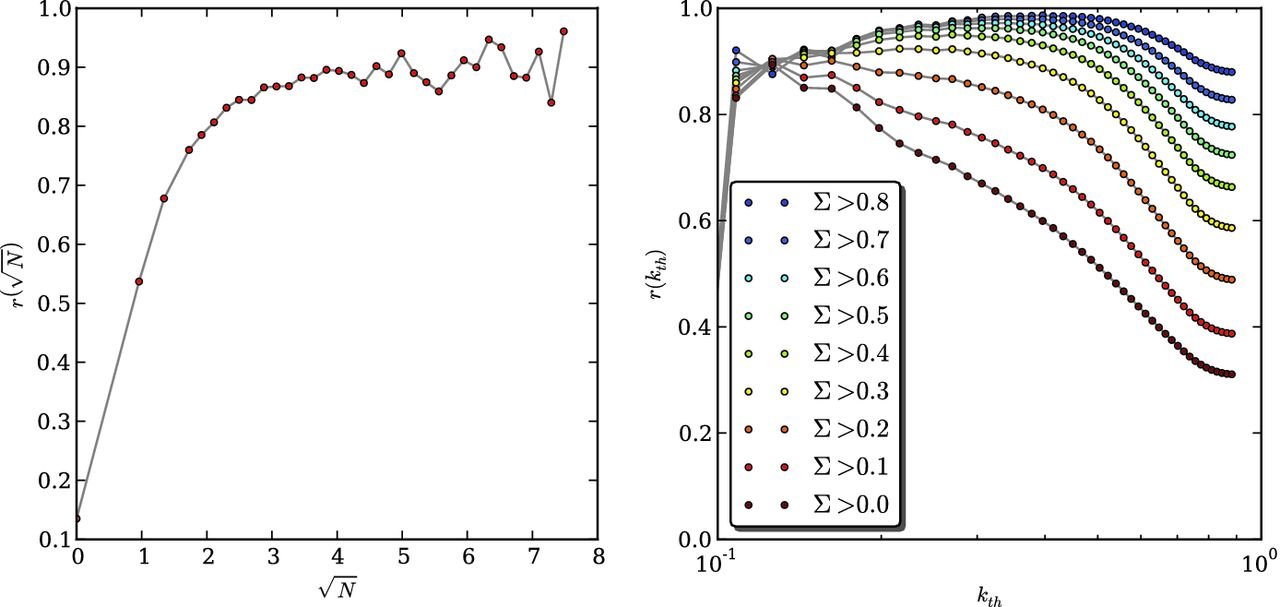
\includegraphics[width=\textwidth]{stt449fig9.jpeg}
        \end{column}
        \begin{column}{0.6\textwidth} % Right column (image)
The correlation coefficient between inferred and real densities is computed as a function of $\sqrt{N}$ for the final and of $k$ for different $\Sigma$ for the initial:
        \begin{center}
        \begingroup\makeatletter\def\f@size{10}\check@mathfonts
$r(k_x)=\frac{\langle\delta_0^x\left\langle\delta\right\rangle^x\rangle}{\sqrt{\left\langle(\delta_0^x)^2\right\rangle}\sqrt{\left\langle(\delta^x)^2\right\rangle}}$
\endgroup
        \end{center}
        \end{column}
    \end{columns}

\end{frame}
\begin{frame}[fragile]{Inferred Dynamics}
True vs inferred dynamics:
\begin{center}
    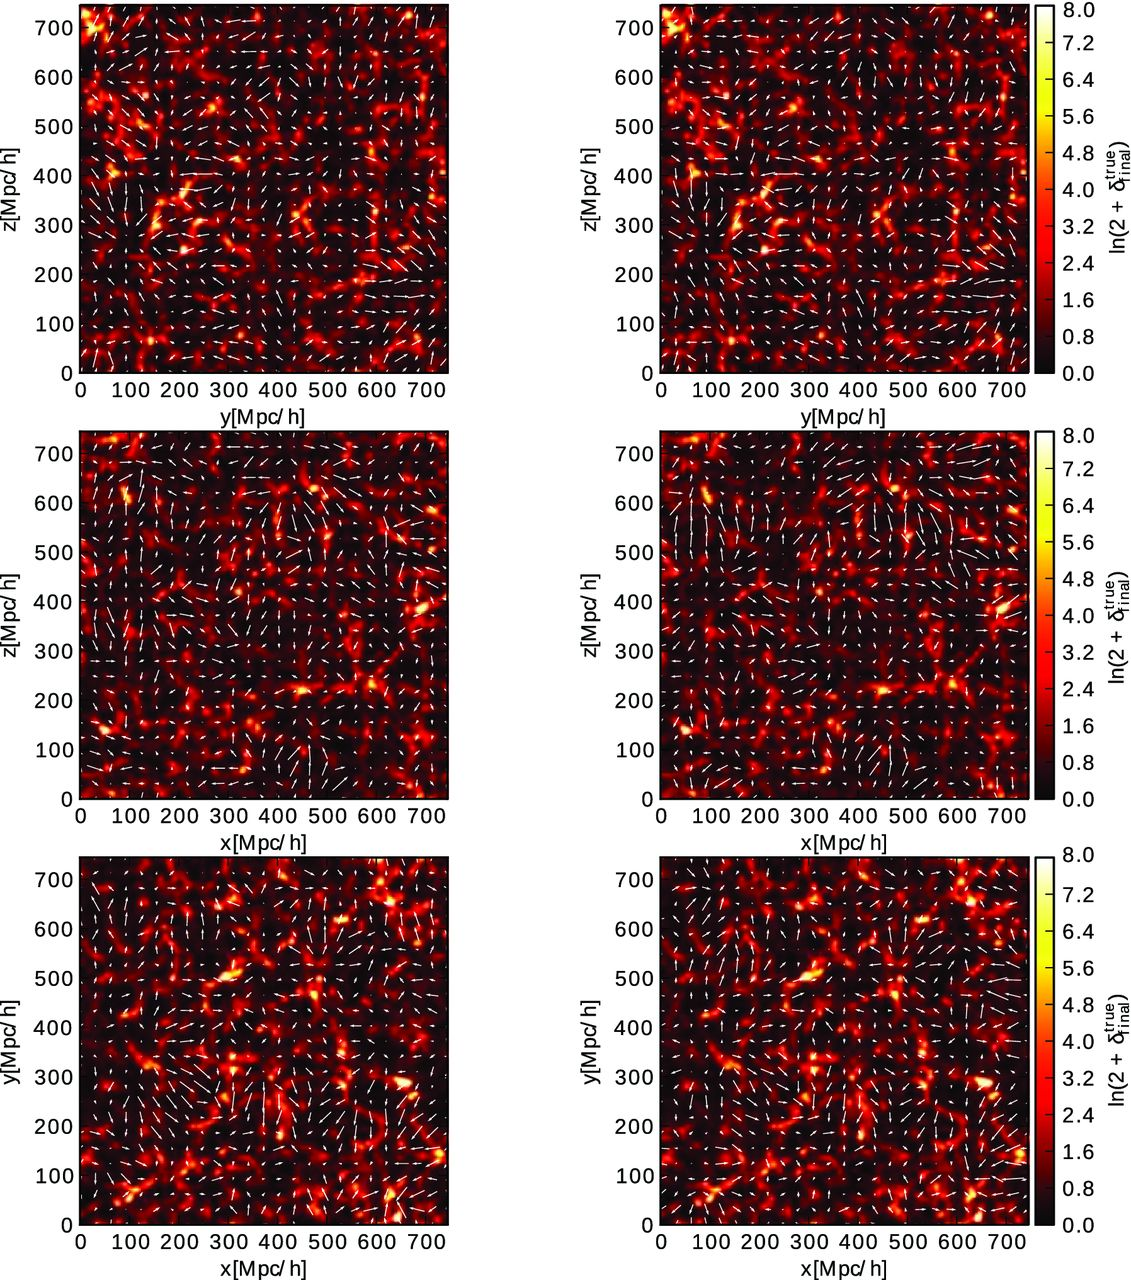
\includegraphics[width=0.55\textwidth]{stt449fig10.jpeg}
\end{center}

  
\end{frame}
\section[Conclusions]{Conclusions}
\begin{frame}[fragile]{Conclusions}
\begin{itemize}
    \item Successfully implemented a forward propagation Bayesian dynamical LSS inference algorithm that correctly accounts for high order statistics in generating initial and final density fields through HMC and 2LPT conditioning on mock data\pause
    \item Achieved low correlation length, short burn - in phase and good mixing, as well as impressive reconstruction capabilities in masked regions\pause
    \item High accuracy in final and initial inferred fields, in particular for high signal-to-noise regions and large scales\pause
    \item Faithful reconstruction of the final density velocity field\pause
    \item Possible further improvements include better model errors and accuracy of 2LPT, real galaxy surveys tests, and incorporation of halo-mode-based galaxy bias models
\end{itemize}
  
\end{frame}
\section[Thank you for your attention]{}

\end{document}
